In order to compute emissions on event or E2O level,
we propose \textit{emission rules} that extract different types of data from an OCEL, and apply a selected emission factor
to determine concrete emissions.

Emission factors are real numbers stating a conversion of a given quantity to \COtwo{} equivalents.
These quantities can be of various units, depending on the activity.
Examples include
\begin{itemize}[itemsep=-1.5ex]
  \item \unit{\kWh} -- electricity from grid,
  \item \unit{\liter} -- fuel combustion,
  \item \unit{\pkm} \textit{(passenger-kilometers)} -- bus transportation,
  \item \unit{\tkm} \textit{(tonne-kilometers)} -- freight.
\end{itemize}

In OCELs, events and objects can be annotated with attribute values.
Each attribute is associated with a specific activity or object type.
The same is adopted for emission rules,
leading to emissions only being computed for events of a given activity.
To compute emissions for multiple activities in the process, multiple emission rules are defined and their results combined.
Moreover, OCELs can contain both attributes with numerical and categorical values.
Here, we only refer to numerical attributes to be used in emission rules.

The units pkm and tkm mentioned above are commonly used for computing transport emissions~\cite{Shirizadeh24climate}.
As they are composed of two quantities by multiplication, emission rules also support multiplying values of different attributes.

\begin{figure}[t]
  \begin{small}
    \begin{center}
      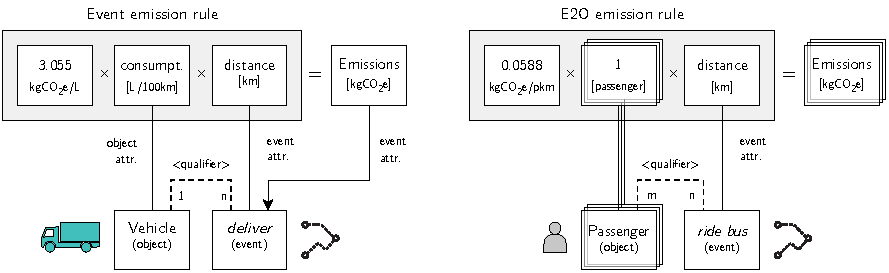
\includegraphics[width=\textwidth]{figures/concept/emission-rule-both-logistics-event-bus-e2o.pdf}
    \end{center}
    \caption{Emission rules using attributes of an event and associated objects. Left: Event emission rule, computing fuel-based emissions in a logistics process. Right: E2O emission rule, computing emission contribution per passenger in a bus transport.}
    % Emission factor sources: GEMIS, UBA\footnotemark}
    \label{fig:emission-rule-both-logistics-event-bus-e2o}
    % event - logistics:
    % ``Diesel - without biofuel content - used in vehicle''
    % https://www.climatiq.io/data/emission-factor/d56128ea-76e5-4a31-a6fe-b5e1ed855e52
    % Germany, GEMIS
    %
    % E2O - bus:
    % ``Emission intensity of diesel urban bus''
    % https://www.climatiq.io/data/emission-factor/06c42852-3f50-4f31-a86c-503d84b3eef5
    % Germany, UBA
  \end{small}
\end{figure}
% https://tex.stackexchange.com/questions/10181/using-footnote-in-a-figures-caption

In \autoref{sec:intro-motiv}, an example for computing emissions delivery events was given,
involving journey distance~[km] and average fuel consumption~[\unit{\liter\per\Ckm}], with example values:

\begin{align*}
	\qty{3.055}{\kgcotwoe\per\liter} \cdot \qty{12.5}{\liter\per\Ckm} \cdot \qty{20}{\km} &= \qty{7.6375}{\kgcotwoe}
  \;(\footnotemark)
\end{align*}
\nopagebreak
\footnotetext{
  \label{fn:factor-diesel-gemis}
  ``Emission intensity of diesel (without biofuel content) per liter used in vehicle''
  -- source: GEMIS
  (\url{https://www.climatiq.io/data/emission-factor/d56128ea-76e5-4a31-a6fe-b5e1ed855e52})
}
%
\autoref{fig:emission-rule-both-logistics-event-bus-e2o}~(left)
shows how this computation is represented by an emission rule:
Attribute values linked to the \otype{vehicle} object (consumption) and the \activity{deliver} event (distance) are multiplied with the emission factor, yielding an emission value for the event.
The result is later integrated into the OCEL as a new event attribute on the \activity{deliver} event.
This is part of the emission allocation framework introduced in \autoref{sec:alloc}.

In this example, emissions are computed on event level.
Still, a vehicle's object attribute value is used.
The value is well-defined because exactly one vehicle participates in the \activity{deliver} event.
Note that attributes of other objects from the logistics process (\autoref{tab:rex-ocel}), such as pallets, cannot be used this way:
The event \ev{deliver}{p2p3} is linked to multiple pallets (\texttt{p2} and \texttt{p3}), making \otype{pallet} a \textit{non-unique type} of the activity \activity{delivery}.

\begin{table}
  \caption{OCEL data usable in emission rules, depending on the level on which emissions are computed. Constant values, attributes of events and those object types uniquely associated with the activity are usable on both levels. E2O rules can additionally include attributes of the object type it is associated with. For the logistics example, the unique types per activity are listed on the right.}
  \label{tab:emission-rules-dtypes}
  \small
  \centering
  \begin{minipage}[t]{.575\textwidth}
    \strut\vspace*{-\baselineskip}\newline
    \begin{tabular}{r@{\ }lcc}
      \toprule
      \textbf{Data type} & & \multicolumn{2}{c}{\textbf{Usable in \dots}} \\
      && \makecell{Event \\ em. rule} & \makecell{E2O \\ em. rule} \\
      \midrule
      Constant && \faCheck & \faCheck \\
      Event attr. && \faCheck & \faCheck \\
      Object attr. & (of E2O object) & {\color{gray}\faTimes} & \faCheck \\
      Object attr. & (of unique type) & \faCheck & \faCheck \\
      Object attr. & (others) & {\color{gray}\faTimes} & {\color{gray}\faTimes} \\
      \bottomrule
    \end{tabular}
  \end{minipage}
  \hfill
  \begin{minipage}[t]{.375\textwidth}
    \strut\vspace*{-\baselineskip}\newline
    \begin{tabular}{rcccc}
      \toprule
      \textbf{Activity} & \multicolumn{4}{c}{\textbf{Unique types}} \\
      & {\color{order} \small\faFileInvoice}
      & {\color{item} \small\faList}
      & {\color{pallet} \small\faBox}
      & {\color{vehicle} \small\faTruck} \\
      & \hspace*{-.5em}{\color{order} \scriptsize ord}\hspace*{-.5em}
      & \hspace*{-.5em}{\color{item} \scriptsize item}\hspace*{-.5em}
      & \hspace*{-.5em}{\color{pallet} \scriptsize pllt}\hspace*{-.5em}
      & \hspace*{-.5em}{\color{vehicle} \scriptsize vhcl}\hspace*{-.5em} \\
      \midrule
      \activity{receive order} & \faCheck &  &  &  \\
      \activity{get item} & \faCheck & \faCheck &  &  \\
      \activity{load} & & {\color{gray}\faTimes} & \faCheck & \faCheck \\
      \activity{deliver} &  &  & {\color{gray}\faTimes} & \faCheck \\
      \activity{inspect} &  &  &  & \faCheck \\
      \bottomrule
    \end{tabular}
  \end{minipage}
\end{table}

In object-centric Petri nets, a process model introduced in OCPM,
this concept is represented by \textit{variable arcs}~\cite{vanderAalst20OCPNs}.
When an object type is not unique for a given activity, the arc between that activity's transition and a place associated with the object type is shown as a double arrow when visualizing the model.
For the logistics OCEL, the different activities' unique and non-unique object types are shown on the right side of \autoref{tab:emission-rules-dtypes}.
Object attributes of non-unique types can only be used by the second type of emission rules, \textit{E2O emission rules}, as shown on the left side of the table.

% , computing emissions on event-to-object (E2O) relation level.
% Here, each emission is linked to an event and an object. This allows 
E2O emission rules compute emissions on the level of E2O relations, with each result linked to an event and an object.
Therefore, the rule is defined for a specific activity and object type.
\autoref{fig:emission-rule-both-logistics-event-bus-e2o}~(right)
depicts such an allocation rule.
The example is from a different process, where multiple \otype{passengers} (represented as objects) are transported by a bus.
To employ an emission factor of the unit \unit{\kgcotwoe\per\pkm}, the passengers are usually counted. E2O emission rules work differently: A count of 1 is used in order to compute individual emission shares per \textit{passenger} object.
Thus, E2O emissions are obtained by
\begin{align*}
	\qty{0.0588}{\kgcotwoe\per\pkm} \cdot \qty{1}{\passenger} \cdot \qty{20}{\km} &= \qty{1.176}{\kgcotwoe}
  \;(\footnotemark).
\end{align*}
\nopagebreak
\footnotetext{
  \label{fn:factor-bus-uba}
  ``Emission intensity of diesel urban bus''
  -- source: UBA
  (\url{https://www.climatiq.io/data/emission-factor/06c42852-3f50-4f31-a86c-503d84b3eef5})
}

% with the emission result corresponding to one individual passenger.
The same computation is carried out for each passenger linked to the \activity{ride bus} event.
In the following step, these values are aggregated in order to obtain total event emissions.
This forms one part of \textit{emission allocation}, presented in the following section.
